\documentclass[conference]{IEEEtran}
\IEEEoverridecommandlockouts
% The preceding line is only needed to identify funding in the first footnote. If that is unneeded, please comment it out.
\usepackage{cite}
\usepackage{amsmath,amssymb,amsfonts}
\usepackage{algorithmic}
\usepackage{graphicx}
\usepackage{textcomp}
\usepackage{xcolor}
\def\BibTeX{{\rm B\kern-.05em{\sc i\kern-.025em b}\kern-.08em
    T\kern-.1667em\lower.7ex\hbox{E}\kern-.125emX}}
\begin{document}

\title{The IIIT Dating App\\
{\footnotesize \textsuperscript{*}Note: Exclusively for IIITians}
\thanks{Identify applicable funding agency here. If none, delete this.}
}

\author{\IEEEauthorblockN{ Dhulipati Lakshmi Girija}
\IEEEauthorblockA{\textit{Computer Science and Engineering} \\
\textit{International Institute of Information Technology}\\
Hyderabad, Telangana \\
lakshmi.dhulipati@students.iiit.ac.in}
}

\maketitle

\begin{abstract}
In this paper we will look into building  dating app exclusively for IIITians who wants to find to fulfill their relationship needs according to their own preferences. We will go into further depth in the matter of recommendations a person might receive and how they might vary according to different relationship preferences.
\end{abstract}

\begin{IEEEkeywords}
Dating, Casual, Long term, Recommendation
\end{IEEEkeywords}

\section{Introduction}
\subsection{The problems with Tinder and Bumble}
There have been many apps in the areas related to dating those including tinder and bumble which act as matchmaking sites. But as any other app, they are flawed and there is a lot of room for improvement, from the recommendation system to the dating styles
\subsection{Emotional connection}
The matchmaking apps considered in our place are purely based on attraction. That is though you might find a person attractive there is no guarantee that you may actually like them. And in terms of long term dating this proves useless. 
\subsection{Communicating expectations}
Considering the problem of not being to efficiently communicate what they expect of their partner whether they're looking for short term commitments or long term commitments or rather casual hookups proves to be useless. 
\subsection{Anonymity}
They don't provide anonymity for the person who chooses to and dictates that everyone must upload a clear photo of themselves. It should be possible for a person to remain anonymous if he/she wishes so by giving them a proper code of identification.
\subsection{Polygamy}
And apps like tinder and bumble unknowingly promote polygamy as it can be seen that 14 percent of their users are on the app for affairs. The app lures people back in to try their hand at it again and again which does more harm than good to long term relationships
\subsection{Likes}
Left swipes and Right swipes prevent going back and viewing the person again even if it a mistake. This clearly needs a change.

\section{Literature Review}

\subsection{Functioning of the apps}
Tinder and Bumble are location based and time based real-time apps. They use the number of likes a person got as a term for popularity and are shown more frequently and at the start of the list when compared to those who gained less likes. They have a scale to adjust the distances up to which you want to find a partner. They provide us with a note make us share something about ourselves.

\subsection{The recommendation system}
Originally any person just registering in the app will be shown in the recommendations and the more the likes they have garnered the more they are likely to be shown in more frequently and in the top of other recommendations.

\subsection{Likes}
There are three types of ways one can react to a person, Like them, Nope them or super like them. Super Like gives us exclusive benefits to speak to the person.

\subsection{Similar problems}
There is e harmony, a website which takes in the information about you and assigns a weight to each and every question you answer. To get exclusive matches it adds upon all the scores and gives a match number and only those who have a match number higher than a particular value tend to appear. They use distance function to assign the matches according to both, but without being able to choose what kind of personality we want. Then there is pure an app that provides anonymity by not displaying the profiles to the user but it breaks down on how we select a long term partner. 

\begin{figure}[htbp]
\centerline{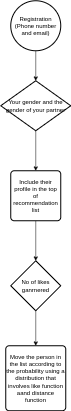
\includegraphics{dass_1.drawio.png}}
\caption{The flow chart for recommendation system}
\label{fig}
\end{figure}

\section{System Architecture}

\subsection{Recommendation}
To make matches based on emotional connection we can use an algorithm which is similar to e harmony. By taking in all the emotional parameters such as IQ, EQ, confidence, and such. Upon taking up all these questions we assign a percentage to it according to the importance of the feature in a relationship and measure it with the other person and give the probability percentage. Taking into account the probability percentage, which we display on top of every match and their compatibility results on various factors for them to compare, we let the user choose how much factor a person wants in the personality using a percentage slide bar option for different factors. If there are many people that list after filtering them, we show the users their potential partners using an inverse exponential distribution with respect to distance and likes. Let number of likes be l. Then the recommendation system to calculate probabilities based on exp(-al). If a person wishes to remain anonymous with repect to few people he/she may provide us with their IIIT mail ID and we exclude the person from being seen by them. The person may also wish to choose the language spoken by the other person.

\subsection{Likes}
Instead of swipe left and right where we can't view the person after swiping once, we can have a list of people with scrolling down or going to the next page as options for viewing them and liking them on wish or removing their like. Instead of super like, we can add them to the favorites page where the person can view exclusively their favorite profiles 

\subsection{Communicating expectations}
Instead of people spending hours of time trying to get through their expectations and getting back dejected, I would propose we have an option to choose which kind of relationship a person wishes to be in and only show them to people who have the same expectations. If a person is looking for a short term dating we show them to those of short term dating and the same applies to long term. If they choose both they will be visible for both of them and will have others of both short term and long term visible to them.

\subsection{Anonymity}
A person may choose to remain anonymous by not wishing to disclose their name or photos in the app, but they still can be matched according to the personality test they have taken earlier. They may wish to enclose their details some time later which will be possible to do so.

\subsection{Polygamy}
To reduce polygamy inside the usage of the app, we could phrase a pop up question of "Do you want to date me" to the other person and if they both consent on it mutually their relationship profiles will be locked and they won't be able to chat with others though they will be able to see them. And their relationship status will change to "Dating". Others might view their profile but can't chat with them. ***IIIT Specific***. They will further not be taken into consideration for matches but they will be visible in currently dating section where a person might get to know if a person has a girlfriend/boyfriend without asking and avoiding awkwardness behind the scenes.

\begin{figure}[htbp]
\centerline{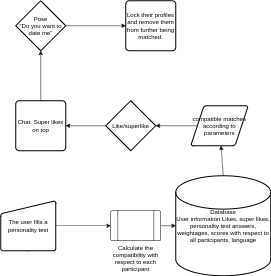
\includegraphics{dass_1.drawio (1).png}}
\caption{Architectural Diagram}
\label{fig}
\end{figure}

\subsection{Login}
The user can register via CAS to make this app IIIT specific. Once the user registers using a username and password, the person may wish to remain anonymous or may upload pictures according to their wish. They may change their birth date, password, or ad but their CAS mail id will remain as the unique identification number.

\subsection{Chat}
The chat feature is enables on liking a person. A person who you give a super like will remain on the top of the chat. The rest all are the same features. Sending emojis, texts, voice calls and video calls options will be provided.

\begin{figure}[htbp]
\centerline{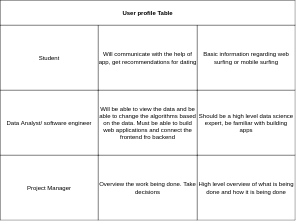
\includegraphics{dass_1.drawio (2).png}}
\caption{User Profile table, actors, usage, familiarity}
\label{fig}
\end{figure}

\begin{figure}[htbp]
\centerline{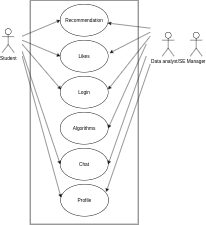
\includegraphics{dass_1.drawio (3).png}}
\caption{Use case diagram}
\label{fig}
\end{figure}

\begin{figure}[htbp]
\centerline{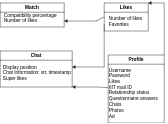
\includegraphics{dass_1.drawio (4).png}}
\caption{Class diagram UML}
\label{fig}
\end{figure}

\begin{figure}[htbp]
\centerline{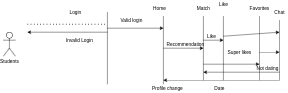
\includegraphics{dass_1.drawio (5).png}}
\caption{Use case sequence}
\label{fig}
\end{figure}

\section*{Conclusion and Further development}

Thus this implementation of the dating app may prove useful to the IIIT students who want to date and are looking for someone with similar tastes or if they want to find if someone they like is already dating or not. We could further improve it by adding a confessions page and dating page where they can put up pictures as a couple and posts page where they can put posts.

\section*{References}

https://www.frontiersin.org/articles/10.3389/fpsyg.2020.01757/full
https://link.springer.com/article/10.1007/s11469-020-00318-9
https://sophia.stkate.edu/cgi/viewcontent.cgi?article=1580&context=msw\_papers
https://www.sciencedirect.com/science/article/pii/S0747563219302961

\end{document}
